\section{Dataset and Experimental Setup}\label{dataset-and-experimental-setup}

SynPEB provides the organized point coordinates and reference plane memberships needed to compare sequential RANSAC, sampled-proposal PEARL, and their hybrid. The experiment separates annotation-based parameter selection from geometric fitting on unseen test scans. This section describes the installed data, preprocessing, evaluation protocol, and metrics. Figs.~\ref{fig:dataset_overview}--\ref{fig:dataset_preprocessing} were generated in MATLAB from fixed training examples, without selecting scans according to algorithm performance.

\subsection{Dataset and annotations}\label{dataset-and-annotations}

The Synthetic Plane Extraction Benchmark (SynPEB), introduced by Schaefer et al. \cite{schaefer2019planes} and distributed with their plane-extraction resources \cite{ppeResources}, contains synthetic organized scans of an indoor environment with polyhedral objects. The published benchmark describes an approximately 6 m \(\times\) 7 m \(\times\) 3 m room, with different plane sizes, orientations, occlusions, and measurement perturbations. It provides 10 training scans and 30 test scans, each organized as 500 \(\times\) 500 measurements. These counts and dimensions agree with the local files.

Each split contains a gt directory and four measurement-variant directories, var1--var4. Thus, the installed archive has 40 reference files and 160 variant files. The experiments process the 40 training and 120 test scan--variant combinations; the gt files support dataset visualization and reference auditing. All four variant names are preserved in reporting. Variants and random seeds derived from the same underlying scan are repeated measurements, not additional independent scenes.

Each PCD record stores x, y, z, and intensity. In these files, intensity encodes the supplied reference ID; it is not used as a reflectance feature. The fitting methods receive coordinates and geometry-based grid information. For evaluation, this project treats IDs \(\geq\) 10 as reference planes and excludes lower IDs from point metrics. Plane IDs identify supports within a scan rather than universal semantic classes. The same numeric ID in another file does not establish correspondence.

\begin{figure*}[!t]
\centering
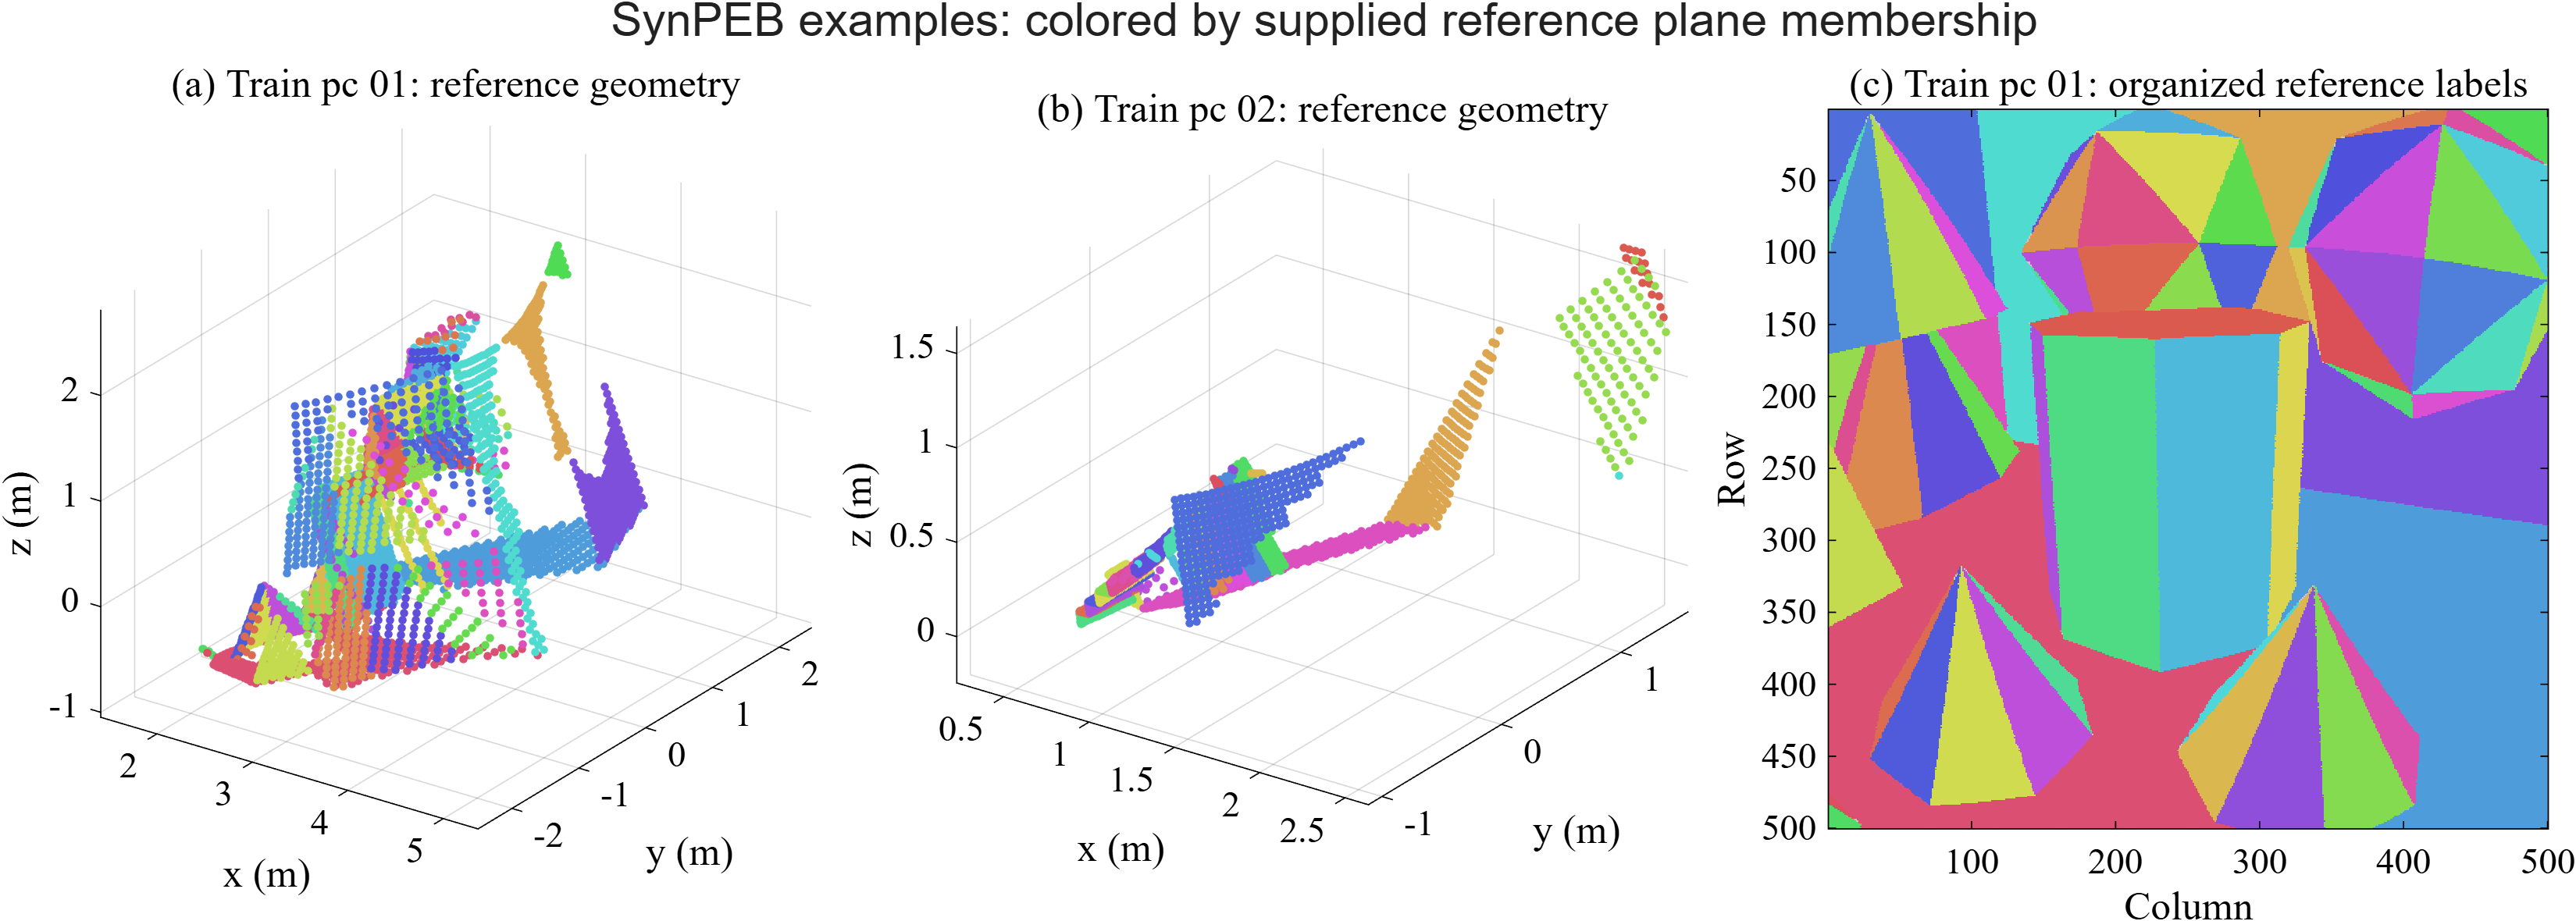
\includegraphics[width=\textwidth]{figures/dataset_overview.png}
\caption{Fixed training examples. Panels (a) and (b) show reference geometry from gt/pc\_01 and gt/pc\_02 at the experimental stride of eight; (c) shows the full-resolution organized label map of gt/pc\_01. Colors denote the supplied plane memberships within each scan and carry no semantic meaning. They are visualization annotations, not algorithm inputs.}
\label{fig:dataset_overview}
\end{figure*}

\begin{figure*}[!t]
\centering
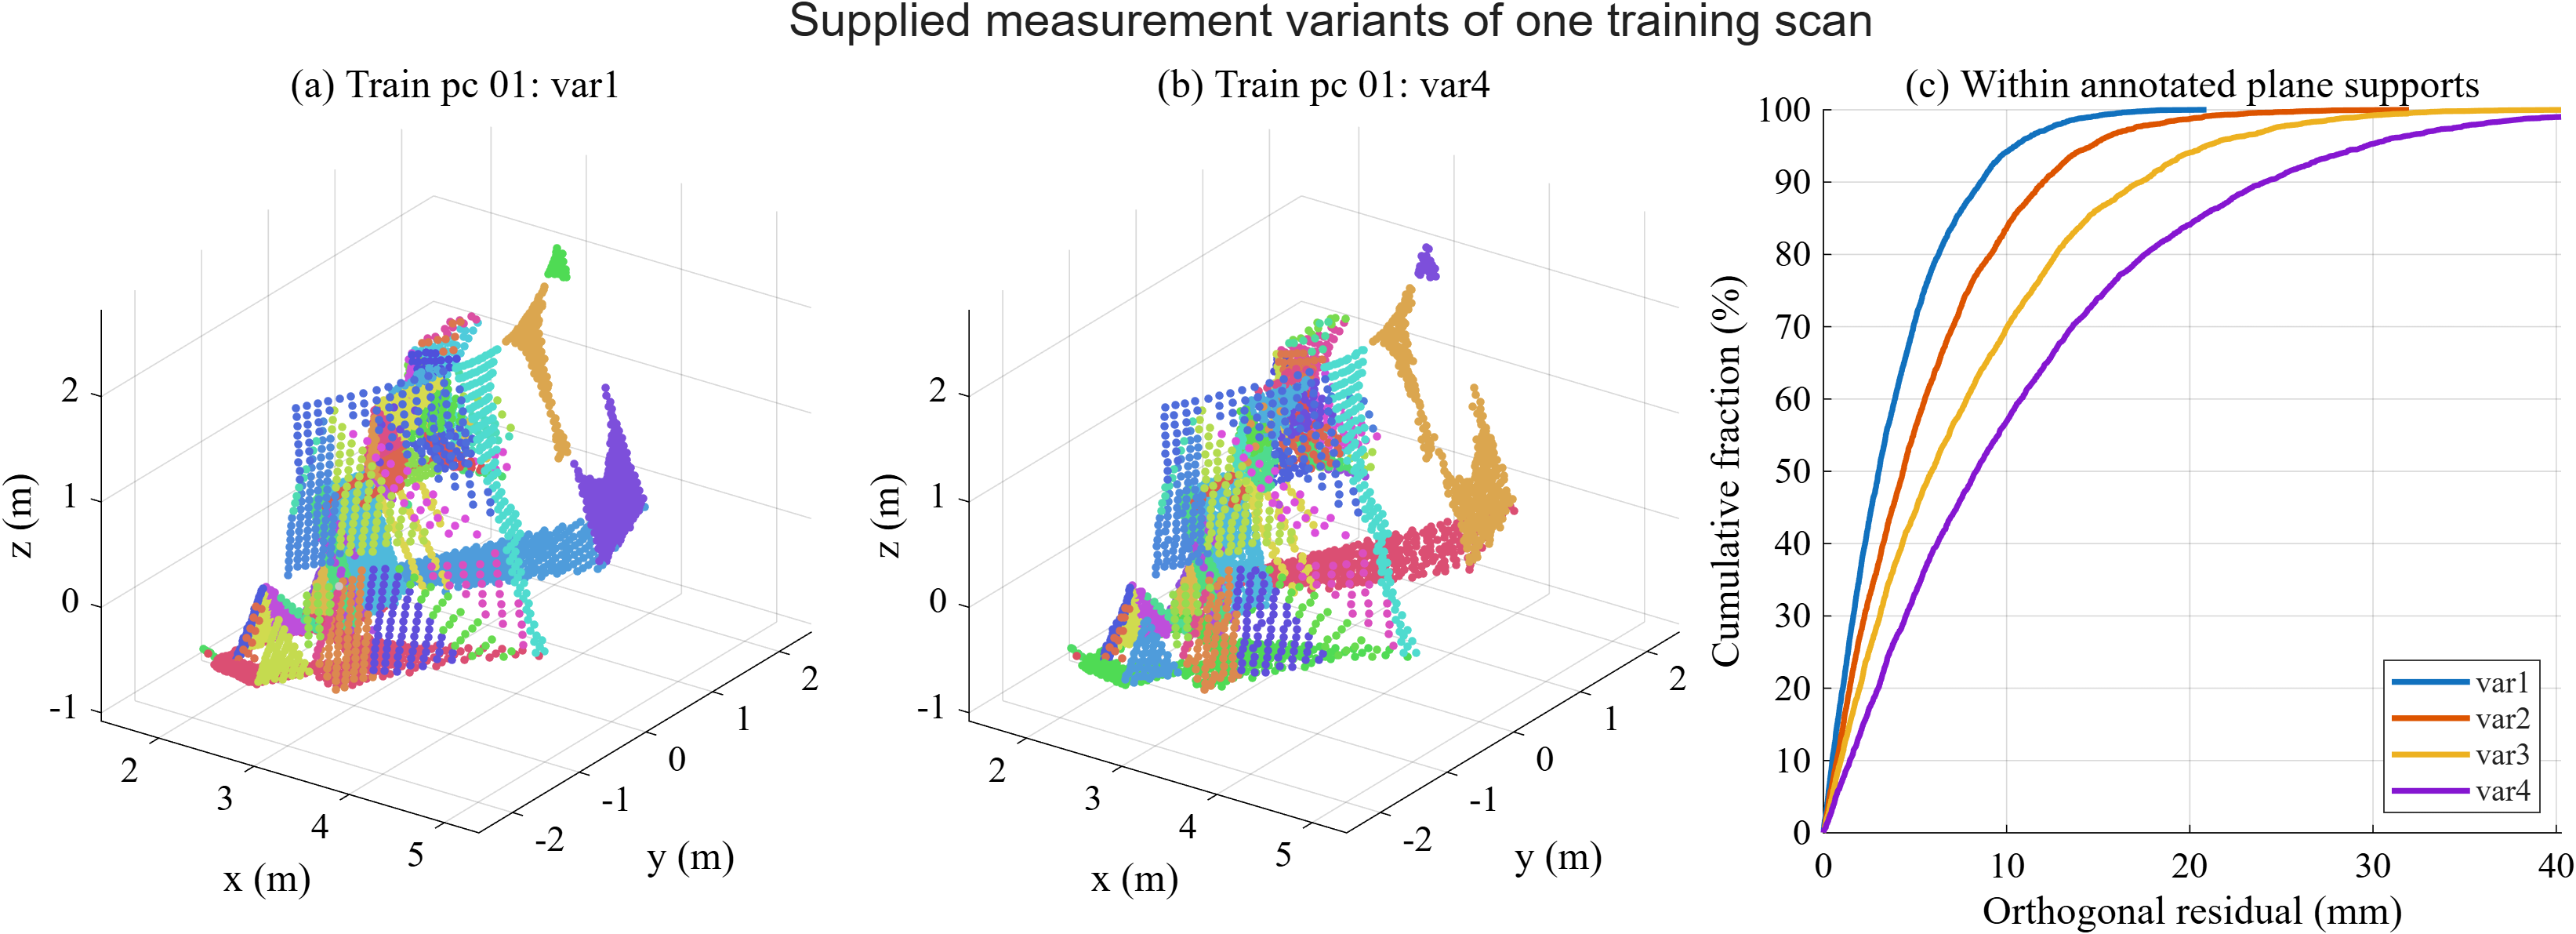
\includegraphics[width=\textwidth]{figures/dataset_variants.png}
\caption{Measurement variants of training scan pc\_01. Panels (a) and (b) use the same view and axis limits, with each file colored using its own annotations. Panel (c) shows cumulative orthogonal residuals after fitting planes to each variant's annotated supports at stride eight. This is a descriptive geometric diagnostic, not an algorithm result or a calibrated estimate of sensor noise. The horizontal range ends at the largest variant-specific 99th percentile; all valid residuals enter each cumulative fraction. Degenerate annotated supports are omitted from this diagnostic.}
\label{fig:dataset_variants}
\end{figure*}

\subsection{Preprocessing and spatial graph}\label{preprocessing-and-spatial-graph}

Point ordering is preserved when decoding the PCD files. The organized row--column index is converted to the corresponding point index before sampling. Every eighth row and column is retained, starting from index one. For a complete 500 \(\times\) 500 scan, this produces 63 \(\times\) 63 = 3,969 points, approximately 1.59\% of the original measurements. Non-finite coordinates and all-zero coordinate records are discarded after sampling. Reference labels follow exactly the same retained indices.

The corresponding variant's own intensity labels provide the evaluation reference; labels are not copied blindly from a same-named gt file. This preserves consistency between the measured coordinates and their supplied annotations. Points excluded by the evaluation mask can still participate in fitting and spatial optimization. The ground-truth mask is not used to select hypotheses, construct neighborhoods, or remove input points.

The PEARL graph joins horizontally and vertically adjacent valid sampled positions, removing edges longer than 0.30 m. Remaining edge weights are \(\exp(-\|x_i-x_j\|_2^2/(2\sigma^2))\), with \(\sigma\) = 0.15 m. For the Fig.~\ref{fig:dataset_preprocessing} example, the graph contains 3,969 nodes and 7,412 edges. Colors in the graph illustration reveal reference supports, while connectivity is computed entirely from geometry. All compared methods use the same sampled cloud; the two PEARL pipelines use the same graph.

\begin{figure*}[!t]
\centering
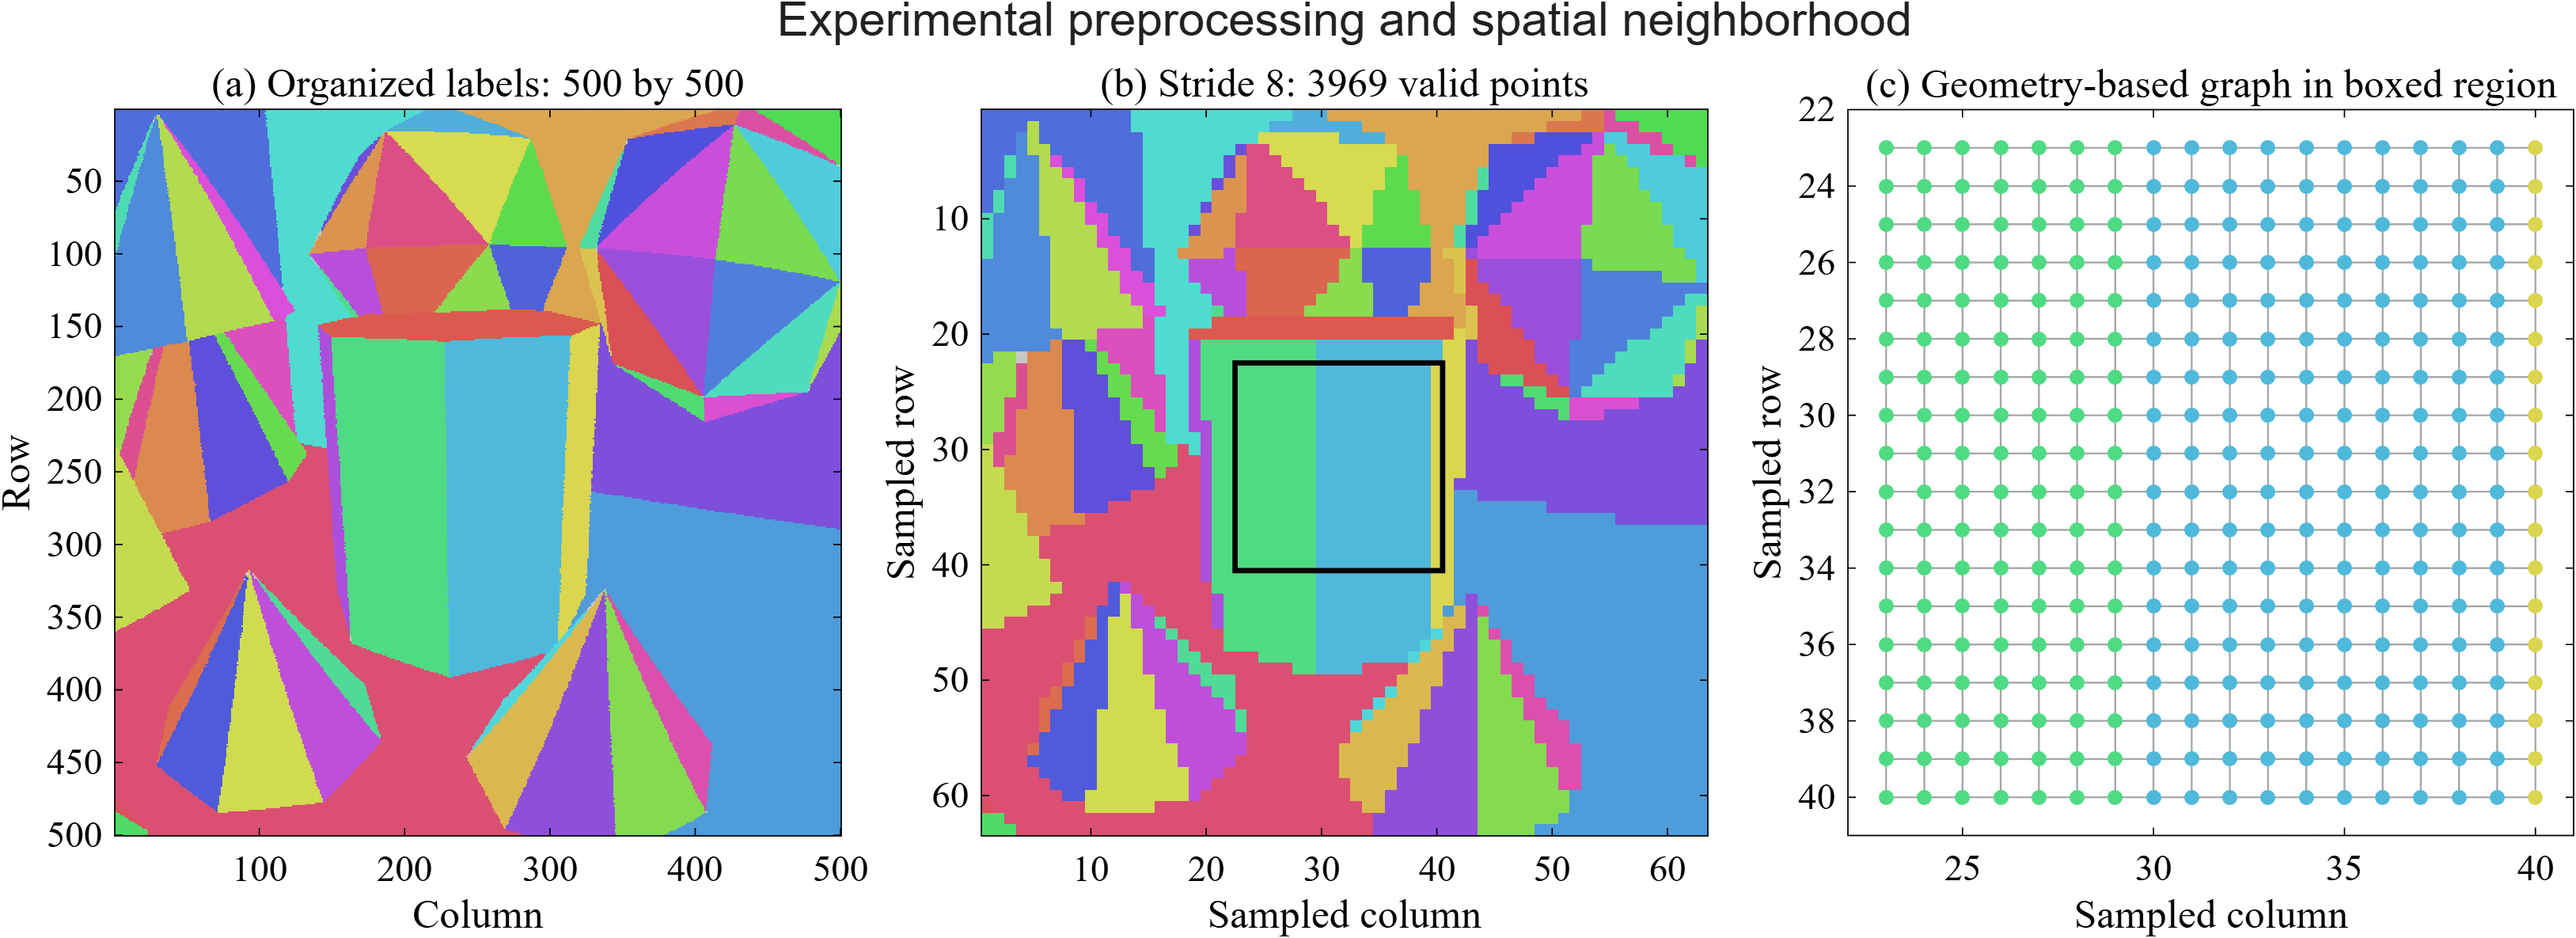
\includegraphics[width=\textwidth]{figures/dataset_preprocessing.png}
\caption{Preprocessing of train/var1/pc\_01. (a) Original organized reference map. (b) The stride-eight grid, with the magnified region boxed. (c) Retained horizontal and vertical neighborhood edges within that region. Edge construction uses grid adjacency and three-dimensional separation, without reference IDs. The annotations are overlaid solely to make the graph's relation to surfaces visible.}
\label{fig:dataset_preprocessing}
\end{figure*}

\subsection{Parameter selection and test protocol}\label{parameter-selection-and-test-protocol}

The training split is used to select hyperparameters, not to learn reusable plane coefficients or classifier weights. Screening evaluates scans 1--2, variants var1 and var4, and seed 7. A staged search varies proposal count, plane cap, and local sampling radius, then examines 25 distance-threshold and smoothness-ratio combinations, followed by minimum support. Previously evaluated configurations are reused. This is a heuristic staged search rather than an exhaustive search over the full parameter product.

The three highest-ranked screened configurations are confirmed on the disjoint training scans 3--10, all four variants, and seeds 7, 19, and 43. This gives 96 scan--variant--seed records per configuration and method. Ranking maximizes the equally weighted average of RANSAC and PEARL mean matched Intersection over Union (IoU; see Section~\ref{evaluation-metrics}); ties use the corresponding mean F1 score (see Section~\ref{evaluation-metrics}), then summed mean runtime. This selection criterion is shared across the two methods, rather than optimized for PEARL accuracy alone.

The confirmed configuration uses 1,000 PEARL proposal attempts, a plane cap of 150, minimum support six, local radius eight, distance threshold 0.04 m, and smoothness ratio 0.4. PEARL permits 15 outer iterations and three expansion sweeps per iteration; the remaining settings follow Sections~\ref{ransac-and-sequential-ransac}--\ref{hybrid-ransac-and-pearl-method}. These values are frozen before testing. The hybrid uses the same settings without separate tuning.

Final testing covers 30 scans \(\times\) 4 variants \(\times\) 3 seeds = 360 records per method. Resetting the generator before each pipeline makes each scan--variant--seed case reproducible. The three methods are evaluated on identical input points. The hybrid starts from the exact standalone RANSAC result, and the no-smoothness ablation uses the sampled PEARL plane bank with the smoothness ratio set to zero. Repeated seeds and variants are correlated; reported means and standard deviations are descriptive across records rather than uncertainty estimates from 360 independent scenes.

\subsection{Evaluation metrics}\label{evaluation-metrics}

Predicted plane numbers have no intrinsic relation to the reference numbers. Let V denote the indices with evaluable reference labels, \(G_{a}\) the support of reference plane a, and \(S_{b}\) the support of predicted plane b restricted to V. Predicted label zero is excluded from the predicted-plane set and denotes rejection. The overlap matrix is

\begin{equation}
C_{ab}=|G_a\cap S_b|.
\label{eq:57}
\end{equation}

A partial one-to-one matching \(\pi\) between reference and predicted planes maximizes total overlap:

\begin{equation}
\pi^*\in\operatorname*{arg\,max}_{\pi}\sum_{(a,b)\in\pi}C_{ab}.
\label{eq:58}
\end{equation}

Matched point accuracy is the fraction of evaluable points assigned to their matched reference plane:

\begin{equation}
\mathrm{Accuracy}=\frac{\sum_{(a,b)\in\pi^*}C_{ab}}{|V|}.
\label{eq:59}
\end{equation}

Rejected reference-plane points and points assigned to unmatched predicted planes count as errors. Unlike many-to-one matching, this rule does not allow several fragments of one reference plane to all receive correct labels. Confusion matrices are computed after matching and saved per case, since plane IDs are scan-specific. Row-normalized displays show within-reference-plane assignment proportions; they do not replace the count-based accuracy calculation.

Intersection over Union (IoU) measures how closely a predicted plane's points match those of a reference plane. It divides the number of evaluable points in both planes (the intersection) by the number in either plane (the union). IoU ranges from 0 for no shared points to 1 for identical point sets. For example, if a reference plane contains 80 points and a predicted plane contains 70 evaluable points, with 60 shared points, their IoU is 60 / (80 + 70 \(-\) 60) \(\approx\) 0.67. For a reference--prediction pair,

\begin{equation}
\mathrm{IoU}_{ab}=\frac{C_{ab}}{|G_a|+|S_b|-C_{ab}}.
\label{eq:60}
\end{equation}

Mean matched IoU uses the same maximum-overlap matching as point accuracy, rather than a matching that directly maximizes IoU:

\begin{equation}
\mathrm{mIoU}=\frac1G\sum_{(a,b)\in\pi^*}\mathrm{IoU}_{ab}.
\label{eq:61}
\end{equation}

Here G is the total number of evaluable reference planes, so unmatched reference planes contribute zero. This macro-average gives each reference plane equal weight, whereas point accuracy gives large supports greater influence. In the saved test cases, the 120 distinct scan--variant inputs contain 9--88 reference planes after sampling, with a mean of 40.93; these counts are not multiplied by the repeated seeds.

Plane-instance detection uses a separate one-to-one matching restricted to pairs with IoU \(\geq\) 0.5. The implementation assigns each eligible edge weight 1 + IoU and maximizes the sum of those weights; accepted pairs define true positives TP. Recall is the fraction of evaluable reference planes that are successfully matched (TP out of G). Precision is the fraction of extracted planes that are successfully matched (TP out of B, where B counts all extracted positive-label planes). The F1 score is the harmonic mean of precision and recall: it is high only when both are high. The three metrics are calculated as follows:

\begin{equation}
\mathrm{Precision}=\frac{\mathrm{TP}}B,\qquad\mathrm{Recall}=\frac{\mathrm{TP}}G,
\label{eq:62}
\end{equation}

\begin{equation}
F_1=\frac{2\,\mathrm{Precision}\,\mathrm{Recall}}{\mathrm{Precision}+\mathrm{Recall}}.
\label{eq:63}
\end{equation}

For example, if 6 of 10 evaluable reference planes are matched and 8 planes were extracted, recall is 6/10 = 0.60 and precision is 6/8 = 0.75, giving an F1 score of about 0.67. Zero denominators are handled explicitly in the implementation. All extracted planes enter B, including planes supported only by ignored points; such a plane cannot match an evaluable reference. A missed plane is an unmatched reference under the detection matching, giving G \(-\) TP. Point errors, mean matched IoU, and instance detection therefore measure different aspects of segmentation quality.

Oversegmentation counts reference planes for which at least two predictions each cover 10\% or more of the reference support. Undersegmentation counts predictions for which at least two reference planes each constitute 10\% or more of their evaluable support. These are project-specific diagnostic definitions and are not assumed identical to the original SynPEB paper's evaluation protocol. The number of extracted planes is also reported.

Algorithm timers exclude data loading, graph construction, reference matching, and figure export. Hybrid total time includes RANSAC initialization once plus PEARL refinement; component times are recorded separately. PEARL histories report the original geometric-plus-spatial energy after initialization, expansion, and refitting. Energy descent verifies progress on the chosen objective but does not by itself establish improved reference accuracy. Mean accuracy across records and point-weighted aggregate accuracy are reported separately.

\subsection{Dataset limitations and scope}\label{dataset-limitations-and-scope}

SynPEB supplies controlled geometric annotations, but its synthetic polyhedral environment does not cover the full diversity of real sensors, material effects, dynamic objects, curved surfaces, and clutter. Performance on these scans therefore supports conclusions about this benchmark and configuration, rather than general real-world robustness. The graph also assumes an organized scan, which limits direct transfer to arbitrary unorganized point clouds.

Stride-eight sampling reduces computational cost while removing small supports and altering neighborhood distances. The number of remaining annotated planes can differ from the original full-resolution count. Results must therefore be compared under the same sampling policy. In addition, finite reference patches are evaluated against models of infinite planes: touching or coplanar regions may be geometrically ambiguous without extra appearance or object information.

Stanford S3DIS \cite{armeni2016s3dis} offers real indoor scans annotated for semantic building elements and objects. These annotations do not directly define a complete plane-instance partition: one object may contain several planar faces, and one semantic class may span many distinct planes. Additional geometric annotation would be needed for the same plane-level matching protocol. SynPEB was chosen to make reference plane membership explicit, while a separately annotated real-data evaluation remains a useful extension.
